\chapter{Длинное название главы, в которой мы смотрим на примеры того, как будут верстаться изображения и списки} \label{chapt2}

\section{Одиночное изображение} \label{sect2_1}

\begin{figure}[ht] 
  \center
  
\includegraphics [scale=0.27] {latex}
  \caption{TeX.} 
  \label{img:latex}  
\end{figure}

%\newpage
%============================================================================================================================
\section{Длинное название параграфа, в котором мы узнаём как сделать две картинки с общим номером и названием} \label{sect2_2}

А это две картинки под общим номером и названием:
\begin{figure}[ht]
  \begin{minipage}[ht]{0.49\linewidth}
    \center{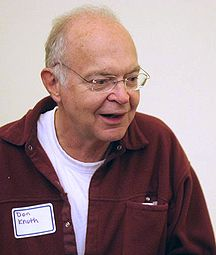
\includegraphics[width=0.5\linewidth]{knuth1} \\ а)}
  \end{minipage}
  \hfill
  \begin{minipage}[ht]{0.49\linewidth}
    \center{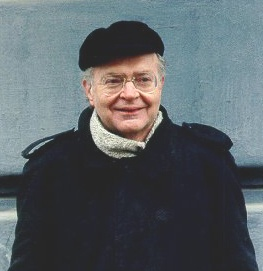
\includegraphics[width=0.5\linewidth]{knuth2} \\ б)}
  \end{minipage}
  \caption{Очень длинная подпись к изображению, на котором представлены две фотографии Дональда Кнута}
  \label{img:knuth}  
\end{figure}

Те~же~две картинки под~общим номером и~названием, но с автоматизированной нумерацей подрисунков посредством пакета \verb|subcaption|:
\begin{figure}[ht]
    \center{
        \hfill
        \subcaptionbox[List-of-Figures entry]{Первый подрисунок\label{img:knuth_2_1}} {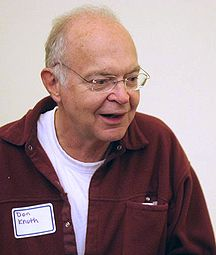
\includegraphics[width=0.25\linewidth]{knuth1}}%
        \hfill       
        \subcaptionbox{Второй подрисунок\label{img:knuth_2_2}} {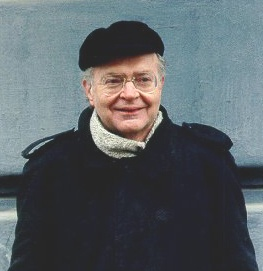
\includegraphics[width=0.25\linewidth]{knuth2}}
        \hfill
    }
    
    \onehalfspacing{% внутри окружения figure набитый текст идёт через одинарный интервал, потому применяем эту команду пакета setspace. Возможно это временный "костыль", до появления соответствующей настройки в преамбуле
    Подрисуночный текст, описывающий обозначения, например. Согласно ГОСТ 2.105, пункт 4.3.1, располагается перед наименованием рисунка.
    }
    \caption{Очень длинная подпись к второму изображению, на котором представлены две фотографии Дональда Кнута} % Этот текст попадает в названия рисунков в списке рисунков
    \label{img:knuth_2}  
\end{figure}


На рисунке~\ref{img:knuth_2_1} показан Дональд Кнут без головного убора. На рисунке~\ref{img:knuth_2}\subref*{img:knuth_2_2}  показан Дональд Кнут в головном уборе.

%\newpage
%============================================================================================================================
\section{Пример вёрстки списков} \label{sect2_3}

\noindent Нумерованный список:
\begin{enumerate}
  \item Первый пункт.
  \item Второй пункт.
  \item Третий пункт.
\end{enumerate}

\noindent Маркированный список:
\begin{itemize}
  \item Первый пункт.
  \item Второй пункт.
  \item Третий пункт.
\end{itemize}

\noindent Вложенные списки:
\begin{itemize}
  \item Имеется маркированный список.
  \begin{enumerate}
    \item В нём лежит нумерованный список,
    \item в котором
    \begin{itemize}
      \item лежит ещё один маркированный список.
    \end{itemize}    
  \end{enumerate}
\end{itemize}


\section{Пробелы}

В~русском наборе принято:
\begin{itemize}
    \item единицы измерения, знак процента отделять пробелами от~числа: 10~кВт, 15~\%;
    \item $\tg 20^\circ$, но: 20~${}^\circ$C;
    \item знак номера, параграфа отделять от~числа: №~5, \S~8;
    \item стандартные сокращения: т.\:е., и~т.\:д., и~т.\:п.;
    \item неразрывные пробелы в~предложениях.
\end{itemize}

\section{Математика}

Русская традиция начертания греческих букв отличается от~западной. Это исправляется серией \verb|\renewcommand|.
\begin{itemize}
    \item[До:] $ \epsilon \ge \phi$, $\phi \leq \epsilon$, $\kappa \in \emptyset$.
    \renewcommand{\epsilon}{\ensuremath{\varepsilon}}
    \renewcommand{\phi}{\ensuremath{\varphi}}
    \renewcommand{\kappa}{\ensuremath{\varkappa}}
    \renewcommand{\le}{\ensuremath{\leqslant}}
    \renewcommand{\leq}{\ensuremath{\leqslant}}
    \renewcommand{\ge}{\ensuremath{\geqslant}}
    \renewcommand{\geq}{\ensuremath{\geqslant}}
    \renewcommand{\emptyset}{\varnothing}
    \item[После:] $\epsilon \ge \phi$, $\phi \leq \epsilon$, $\kappa \in \emptyset$.
\end{itemize}

Кроме того, принято набирать греческие буквы вертикальными, что решается подключением пакета \verb|upgreek| и~аналогичным переопределением в преамбуле.


\section{Кавычки}
В английском языке приняты одинарные и двойные кавычки в~виде ‘...’ и~“...”. В России приняты французские («...») и~немецкие („...“) кавычки (они называются «ёлочки» и~«лапки», соответственно). <<Лапки>> обычно используются внутри ,,ёлочек'', например, <<... наш гордый ,,Варяг``...>>.

Французкие левые и правые кавычки набираются
как лигатуры \verb|<<| и \verb|>>|, а~немецкие левые и правые кавычки набираются как лигатуры \verb|,,| и \verb|‘‘| (\verb|``|).

Вместо лигатур или команд с активным символом "\ можно использовать команды \verb|\glqq| и \verb|\grqq| для набора немецких кавычек и команды \verb|\flqq| и \verb|\frqq| для набора французских кавычек. Они определены в пакете \verb|babel|.

\section{Тире}
%  babel+pdflatex по умолчанию, в polyglossia надо включать опцией (и перекомпилировать с удалением временных файлов)
Команда \verb|"---| используется для печати тире в тексте. Оно несколько короче английского длинного тире. Кроме того, команда задаёт небольшую жёсткую отбивку от слова, стоящего перед тире. При этом, само тире не отрывается от слова. После тире следует такая же отбивка от текста, как и перед тире. При наборе текста между словом и командой, за которым она следует, должен стоять пробел.

В составных словах, таких, как <<Закон Менделеева"--~Клапейрона>>, для печати тире надо использовать команду \verb|"--~|. Она ставит более короткое, по~сравнению с английским, тире и позволяет делать переносы во втором слове. При~наборе текста команда \verb|"--~| не отделяется пробелом от слова, за которым она следует (\verb|Менделеева"--~|). Следующее за командой слово может быть  отделено от~неё пробелом или перенесено на другую строку.

Если прямая речь начинается с абзаца, то перед началом её печатается тире командой
\verb|"--*|. Она печатает русское тире и жёсткую отбивку нужной величины перед текстом.

\section{Дефисы и переносы слов}
%  babel+pdflatex по умолчанию, в polyglossia надо включать опцией (и перекомпилировать с удалением временных файлов)
Для печати дефиса в составных словах введены две команды. Команда~\verb|"~| печатает дефис и~запрещает делать переносы в~самих словах, а~команда \verb|"=| печатает дефис, оставляя \TeX ’у право делать переносы в~самих словах.

В отличие от команды \verb|\-|, команда \verb|"-| задаёт место в~слове, где можно делать перенос, не~запрещая переносы и~в~других местах слова.

Команда \verb|""| задаёт место в слове, где можно делать перенос, причём дефис при~переносе в~этом месте не~ставится.

Команда \verb|",| вставляет небольшой пробел после инициалов с правом переноса в фамилии.


\clearpage
